\chapter{Implementation and Testing}
This chapter will first introduce the most significant frameworks that must be installed to be able to run \gls{NDN} applications.
Then the various designs and implementation choices will be explained.
The source code is left out from the appendix due to the size inconvenience. 
Finally, the test result will be presented.

\section{Installing Named Data Networking Protocol}

There are several libraries that is required for experimenting in a \gls{NDN} environment.
Installation guides can be found at the Github project~\cite{ndn-git}.
First we need to install the \gls{ndn-cxx}.
\gls{ndn-cxx} is a implementation of \gls{NDN} primitives. 
It is a fundamental framework that \gls{NDN} application requires. 
Second we need to install the \gls{NFD}~\cite{nfd} which is a network forwarder and also in the core implementation of \gls{NDN}.
The major modules implemented in \gls{NFD} is:
\begin{itemize}
  \item Core - Common services shared between the different \gls{NFD} modules (such as hash, \gls{DNS} resolver, face monitoring etc.).
  \item Faces - Generalization of different interfaces, explained in~\autoref{ndn-node-modules}.
  \item Tables - \gls{PIT}, \gls{CS}, \gls{FIB}, explained in~\autoref{ndn-node-modules}.
  \item Forwarding - Packet processing.
  \item Management - Enables users/programs to interact with the \gls{NFD} forwarder state.
  \item\gls{RIB} Management - Managing routing protocols and application prefix registration.
\end{itemize}
The \gls{NDN} project is under development, and thus the implementation of \gls{NFD} has its deficiencies.
Ideally we want the devices to communicate directly with each other using WiFi, without running over \gls{IP}. 
This face functionality is not yet implemented, and thus \gls{NDN} is running over \gls{IP} in my experiments.

\subsection{Installing PyNDN2}
The work done in this thesis is written in Python, hence the \gls{PyNDN2}~\cite{pyndn2-git} is used.
This is an easy to use implementation of \gls{NDN} and comes with great code examples.

Because the \gls{NDN} protocol require signing of \gls{data} packets (\autoref{ndn-security}) some new implementation in the \gls{PyNDN2} source code was necessary to be able to sign and verify with \gls{IBS}.
I added the \path{python/pyndn/sha256_with_ibswaters_signature.py} file that follows the pattern of the existing RSA Signature (\path{python/pyndn/sha256_with_rsa_signature.py}) and is of type \texttt{Signature}.
Some small additions in the \path{python/pyndn/encoding/tlv_0_1_1_wire_format.py} and the \path{python/pyndn/encoding/tlv/tlv.py} is added so \gls{PyNDN2} recognizes the \gls{IBS} when the \gls{data} packet is encoded and decoded.

\section{Installing Identity-Based Cryptography}
To be able to run \gls{IBC} the \gls{PBC}~\cite{ben2007implementation} needs to be installed.
I use the Charm framework~\cite{charm13} implements several \gls{IBE} and \gls{IBS} schemes in Python.
Charm is a framework for rapidly prototyping cryptosystems.


Some small modifications had to be done in the Waters-\gls{IBS}~\cite{DBLP:journals/iacr/Waters04} implementation in Charm.
In \path{charm/schemes/pksig/pksig_waters.py} there is a global variable, i.e. \texttt{waters}, that is used throughout all the methods in \path{pksig_waters.py}.
The problem is that this variable is declared in the \texttt{setup()}, which is only called at \gls{PKG}, and not by another devices that do not play the role of a \gls{PKG}. 
And thus, the declaration of \texttt{waters} must be moved to the \texttt{\_\_init\_\_()} in \path{pksig_waters.py}.


\section{File Synchronization Module - Implementation}
\gls{FSM} is a python application that runs over \gls{NDN} and synchronizes all files in a specified path, with all participants within the synchronization room.
Application goals are explained in~\autoref{file-sync}.
The module is highly based on the Python implementation of ChronoSync~\cite[test-chrono-chat.py]{pyndn2-git}.
The code can be retrieved from the thesis work repository~\cite[fileSync.py]{garseg15}

The implementation of the \gls{FSM} does not use \gls{IBS}. 
This is because all packets that are sent is managed by ChronoSync. 
ChronoSync uses the PyNDN2 KeyChain to sign and verify all \gls{interest} and \gls{data} packets.
I do however demonstrate that it works perfectly fine to perform both \gls{IBE} and \gls{IBS} over \gls{NDN} in the \gls{HSS} implementation.

The module triggers synchronization when files that are watched is changed, or when a file is added or removed.
A library that makes it possible to watch files in OS X, Linux or Windows, is Watchdog~\cite{watchdog}. 
The implementation is illustrated in the class FileWatch in~\autoref{fig:code-topology}.

\section{Health Sensor System - Implementation}
The \gls{HSS} is a python application that runs over \gls{NDN}.
Application flow is explained in~\autoref{sensor-application}.
The implementation does not deal with sensor data retrieval from actual sensors, nor deal with sending instructions from devices to each other, but rather focuses on the trust model and security in protocols between devices in the network.
The code is divided into several pieces shown in~\autoref{fig:code-topology}.

The Device class~\cite[device.py]{garseg15} implements the role of a device that can express \gls{interest} and offer \gls{data}.
The PKG class~\cite[publicKeyGenerator.py]{garseg15} implements the role of a \gls{PKG}.
Both classes uses \gls{PyNDN2} and IndetityBasedCryptography. 
IdentityBasedCrypto~\cite[identityBasedCrypto.py]{garseg15} implements two \gls{IBE} schemes and one \gls{IBS} scheme. 
These schemes are listed below:
\begin{description}
  \item[Waters05]~\cite{DBLP:journals/iacr/Naccache05} that is a variant of Brent Waters \gls{IBE} scheme~\cite{DBLP:journals/iacr/Waters04}, but with smaller key size, hence more practical.
  \item[Waters09]~\cite{DBLP:conf/crypto/Waters09} that is also a fully secure implementation of \gls{IBE} scheme.
  \item[Waters]~\cite{DBLP:journals/iacr/Waters04} that is a implementation of \gls{IBS} scheme.
\end{description}

\begin{figure}[ht]
  \centering
  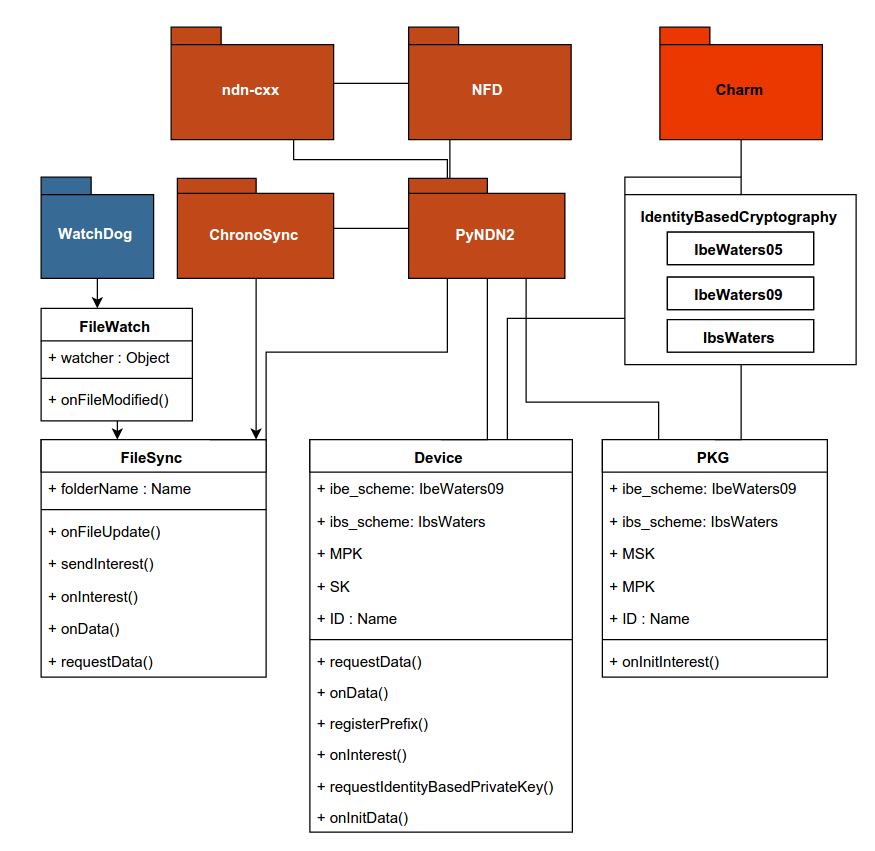
\includegraphics[width=1\textwidth]{code-topology.png}
  \caption[Class topology]{Package and slass topology related to the work done in conjuction to this thesis.}
  \label{fig:code-topology}
\end{figure}

\subsection{Key Management}
Sufficient key management is not implemented.
Storing of secret keys should be done in a secure fashion.

\subsection{Name Structure}
The \gls{ID} of every device is a part of the \gls{name}.
A device register the prefix \path{/ndn/no/ntnu/<device>/<resource>} and hence its \gls{ID} is \path{/ndn/no/ntnu/<device>}.
\todo{more..}

\subsection{Access Control}
In~\autoref{access_control} I present a possible solution for access control.
This is however not implemented in the application, because it is considered too high workload for this thesis.

\subsection{Packet Design}
The packet format is designed with Google Protocol Buffers, which is a language-neutral, platform-neutral, extensible mechanism for serializing structured \gls{data}.\footnote{Google Protocol Buffers - https://developers.google.com/protocol-buffers/}
Initialization packets have the structure presented in~\autoref{fig:init_interest-data}.
Initially the idea was to have the \gls{TMPK} appended to the content \gls{name}. 
However, I experienced a problem where the \texttt{Init} \gls{data} never arrived at destination node. 
After some research in \texttt{ndn-cxx} documentation I found that the packets have a \texttt{MAX\_NDN\_PACKET\_SIZE} of 8800 bytes and the \texttt{Init} \gls{data} exceeded this limit and reached 8904 bytes.
Because the \gls{TMPK} is approximately 2\gls{KB} and was appended to the content \gls{name} in the \gls{interest}, the \gls{data} response off course had to have the same content \gls{name}, hence 2\gls{KB} overhead in the \gls{name}. 
The \gls{TMPK} can as easily be appended to the KeyLocator \gls{name}, hence the \gls{data} response can be 2\gls{KB} less, resulting to a 6866 bytes \texttt{Init} \gls{data} packet.

Sensor packets have the structure presented in~\autoref{fig:sensor_interest-data}.
The code can be reviewed in~\cite[messageBuf.proto]{garseg15}.
\begin{description}
	\item[\texttt{Init} \gls{interest}] - 
  The \texttt{Init} \gls{interest} can be seen in~\autoref{fig:init_interest-data} and consist of three fields: Content Name, KeyLocator and MustBeFresh.
  KeyLocator can be of type \gls{name}. 
  As described in the \gls{NDN} Packet Format~\cite{ndnpacketformat}, generally this field can be used to specify where to download the certificate used to sign the \gls{interest}.
  However, in the trust model I use this field to publish the requesters \gls{name}, i.e. the requesters public key. 
  This is very useful when using \gls{IBE} and \gls{IBS}.
	\item[\texttt{Init} \gls{data}] - 
  The \gls{data} response to the \texttt{Init} \gls{interest} is illustrated in~\autoref{fig:init_interest-data}.
	\item[\texttt{Sensor} \gls{interest}] -
	As in the \texttt{Init} \gls{interest} the KeyLocator field is used to define the ID\textsubscript{requester}. 
  The packet is illustrated in~\autoref{fig:sensor_interest-data}.
	\item[\texttt{Sensor} \gls{data}] - 
  The \gls{data} response to the \texttt{Sensor} \gls{interest} uses the same structure as the \texttt{Init} \gls{data}. 
  It is illustrated in~\autoref{fig:sensor_interest-data}
\end{description}

The \texttt{Init} and \texttt{Sensor} \gls{data} responses in the \gls{HSS} have a structure that is defined in~\cite[messageBuf.proto]{garseg15}.
The fields are:
\begin{itemize}
  \item \texttt{MessageType} is an \texttt{enum} and can be either Init or Sensor.
  \item \texttt{EncAlgorithm} is an \texttt{enum} and represents which type of encryption scheme is used on the content.
  \item \texttt{IbeAlgorithm} is an \texttt{enum} and represents which type of \gls{IBE} scheme is used on the \gls{CEK}.
  \item \texttt{IbsAlgorithm} is an \texttt{enum} and represents which type of \gls{IBS} scheme is used to sign the \gls{data}.
  \item \texttt{MasterPublicKey} is the \gls{PKG}s public parameters used to do \gls{IBE}.
  \item \texttt{SignatureMasterPublicKey} is the \gls{PKG}s public parameters used to do \gls{IBS}.
  \item \texttt{SymmetricKey} is the symmetric key used to encrypt the content. The key is encrypted.
  \item \texttt{Cipher} is the encrypted content.
  \item \texttt{Session} is a nonce.
\end{itemize}

\begin{figure}[ht]
  \centering
  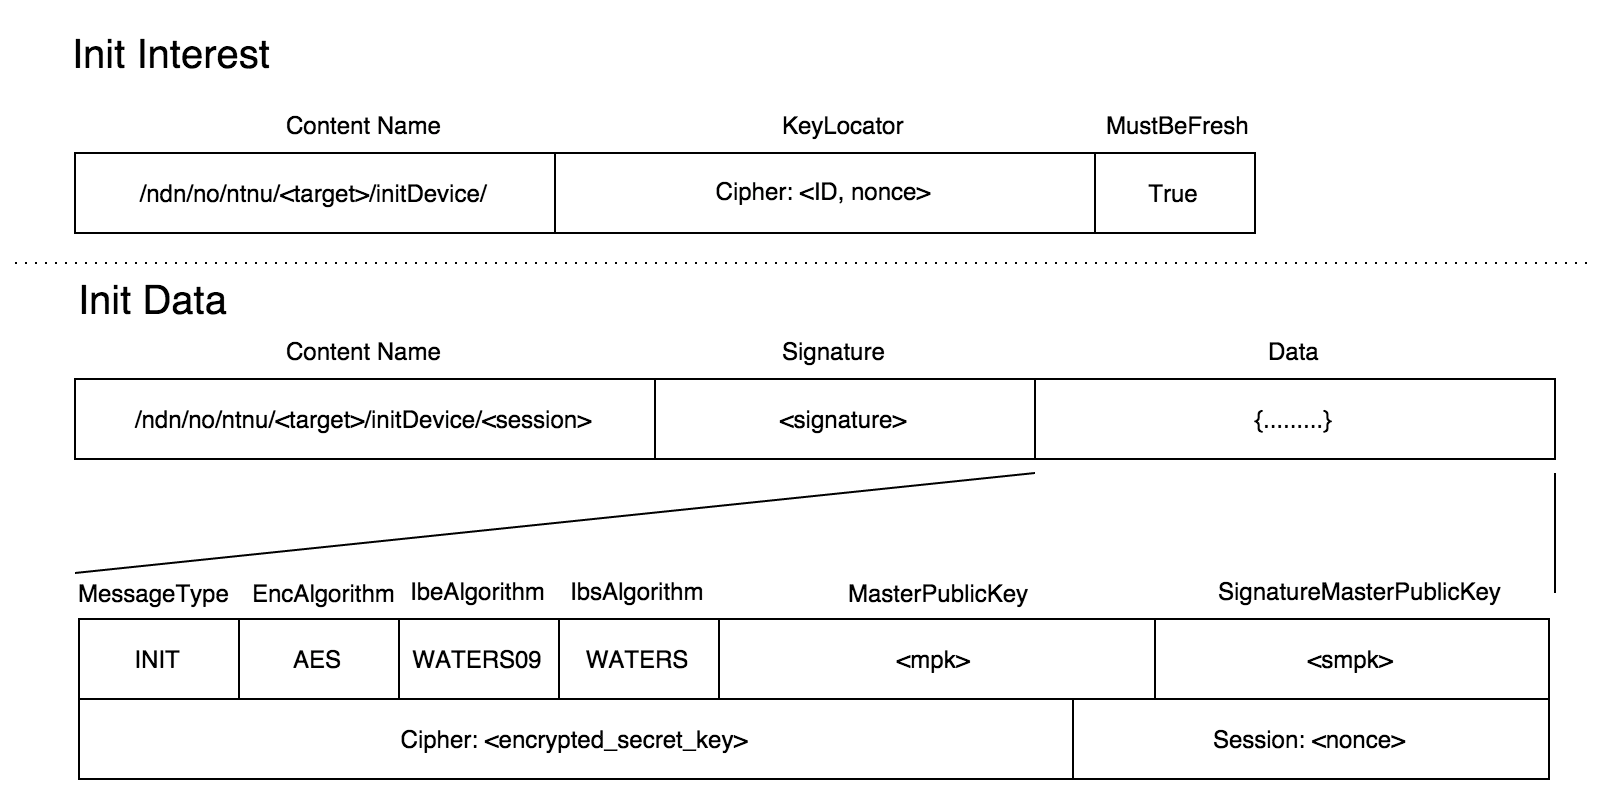
\includegraphics[width=1\textwidth]{init_interest-data.png}
  \caption[Init Interest and Data packet]{\texttt{Init} \gls{interest} and \gls{data}}
  \label{fig:init_interest-data}
\end{figure}

\begin{figure}[ht]
  \centering
  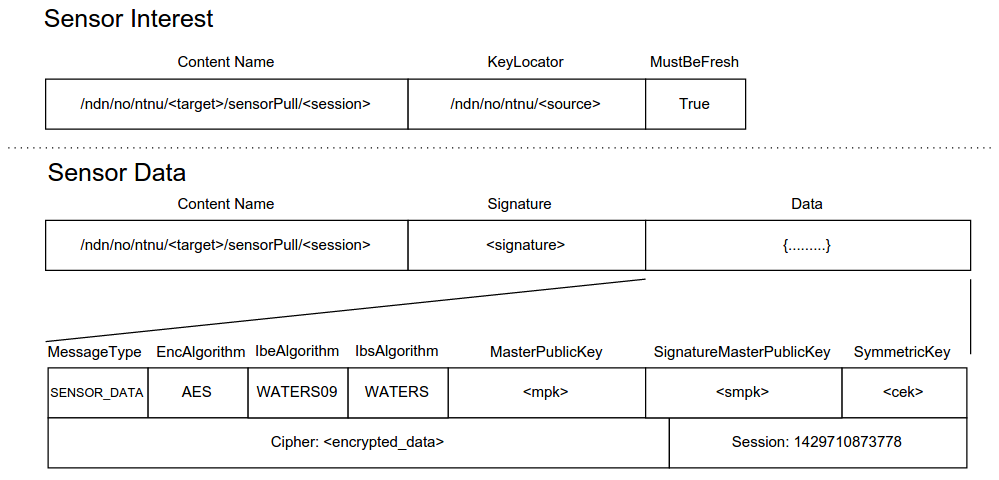
\includegraphics[width=1\textwidth]{sensor_interest-data.png}
  \caption[Sensor Interest and Data packet]{\texttt{Sensor} \gls{interest} and \gls{data}}
  \label{fig:sensor_interest-data}
\end{figure}

\subsection{Running the Code}
First the \gls{NFD} must be started on each device shown in~\autoref{lst:nfd-start}, if not already running. 
Then we have to make sure that each device participating in the network know the \gls{name} and \gls{IP} address binding, since the testing will run \gls{NDN} over \gls{IP}.
This is accomplished by registering the mapping in the \gls{FIB} at each device showed in the second line in~\autoref{lst:nfd-start}.

On the device playing the role of the \gls{PKG}, run the code presented in~\autoref{lst:pkg}. 
This will create the key pair MPK\textsubscript{pkg} and MSK\textsubscript{pkg} and register the prefix where the other nodes can find the \gls{PKG}.

On the device playing the role of e.g. a sensor, run the code presented in~\autoref{lst:data}.
This will automatically register the prefix of the sensor, and start the initialize protocol with the \gls{PKG}.

On the device playing the role of the user device (e.g. a mobile), run the code presented in~\autoref{lst:pull}.
This will automatically start the initialize protocol with the \gls{PKG}.
Running \texttt{r} will make the device expressing an \gls{interest} for sensor \gls{data} from the sensor.

\begin{lstlisting}[language=bash, caption={NFD Start}, label={lst:nfd-start}]
  $ nfd-start
  $ nfdc register /ndn/no/ntnu/<data-device> udp://<device-ip-address>
  $ nfdc register /ndn/no/ntnu/<pull-device> udp://<device-ip-address>
  $ nfdc register /ndn/no/ntnu/<pkg> udp://<pkg-ip-address>
\end{lstlisting}

\begin{lstlisting}[language=bash, caption={Start PKG}, label={lst:pkg}]
  $ python application.py
  $ pkg
\end{lstlisting}

\begin{lstlisting}[language=bash, caption={Start a device registering a prefix.}, label={lst:data}]
  $ python application.py
  $ data
\end{lstlisting}

\begin{lstlisting}[language=bash, caption={Start a device that will express \gls{interest} in \gls{data}.}, label={lst:pull}]
  $ python application.py
  $ pull
  $ r
\end{lstlisting}

\section{Testing}
In this section it will be presented which computers will be used during testing. 
The measurement results will be presented together with the key/content sizes related to the \gls{HSS}.

\subsection{Computers}
The plan was to test the application with several Raspberry Pi's to simulate a sensor network, with limited computation power.
However this is not possible with the Charm framework as it is not compatible with ARM processors.
The \gls{HSS} is tested over several computers presented in~\autoref{tbl:target_computers}.
Each computer is assigned an ID which will be used for reference in the performance measurements.

\begin{table}[h]
  \begin{tabular}{llll}
  ID      & Computer                  & Operating System          & Processor                    \\ \hline
  C1      & Macbook Pro               & 64-bit OS X 10.10         & Intel Core i7 @ 2.0GHz       \\ %\hline
  C2      & Garsbook                  & 64-bit Ubuntu 14.04 LTS   & Intel Core i5 @ 3.0GHz       \\ %\hline
  C3      & HP                        & 64-bit Ubuntu 14.04 LTS   & Intel Core i7 @ 2.8GHz       \\ %\hline
  \end{tabular}
  \caption[Test computers]{Computers used during tests.}
  \label{tbl:target_computers}
\end{table}

\subsection{Key Sizes}
It is listed in~\autoref{tbl:size_chart} the different sizes for keys related to the \gls{IBE} and \gls{IBS} that is used in the \gls{HSS} implementation.
The \gls{CEK} is generated as a group element and is extracted to 40 bytes when performing encryption and decryption with \gls{AES}.
I would prefer to encrypt and send the extracted version of the \gls{CEK}, i.e. the hash value of 40 bytes, but the \gls{IBE} encryption scheme demands a certain type of format on the \gls{data}, and thus the whole \gls{CEK} must be sent.
The \gls{CEK} is a random $\mathbb{G}_T$ element (\autoref{ibe-secureness}), and is generated with \texttt{group.random(GT)}.
\begin{table}[h]
  \begin{tabular}[c]{p{0.4\textwidth}p{0.2\textwidth}p{0.2\textwidth}}
  Data                            & Scheme          & Size              \\ \hline
  Content Encryption Key (CEK)    & Hash($\mathbb{G}_T$) & 244 bytes         \\ %\hline
  IBE Master Public Key           & Waters09        & 2014 bytes        \\ %\hline
  IBE Secret Key (SK)             & Waters09        & 1164 bytes        \\ %\hline
  IBE Encrypted CEK               & Waters09        & 1472 bytes        \\ %\hline
  Encrypted SK                    & AES             & 1633 bytes        \\ %\hline
  IBS Master Public Key           & Waters          & 2360 bytes        \\ %\hline
  IBS Secret Key (SSK)            & Waters          & 260 bytes         \\ %\hline
  IBS Signature                   & Waters          & 412 bytes         \\ %\hline
  Encrypted SSK                   & AES             & 437 bytes         \\ %\hline
  \end{tabular}
  \caption[Size chart of IBC parameters]{Sizes of different keys used in the health sensor system implementation.}
  \label{tbl:size_chart}
\end{table}


\subsection{Performance}\label{ibc-performance}
To be able to evaluate if \gls{IBC} is applicable to devices with small computation power and limited battery, it has to at least perform somewhat in the range of regular asymmetric encryption (read RSA), and signing. 
Naccache suggested that if the prime \gls{p} is 1024-bit, the scheme would provide equivalent security as a RSA 1024-bit key.
For comparison reasons, the RSA key pair is therefore generated with the size of 1024-bit.
In~\autoref{tbl:time_chart} the results from running different cryptographic methods on the computers listed in~\autoref{tbl:target_computers} are presented.

\begin{table}[h]
  \begin{tabular}[c]{lllll}
  Method                                      & Scheme          & C1              & C2          & C3              \\ \hline
  IBE PKG key pair generation                 & Waters09        & 99.65 ms        & 27.09 ms    & 36.08 ms     \\ %\hline
  IBE Secret Key (SK) generation              & Waters09        & 56.14 ms        & 17.86 ms    & 23.27 ms     \\ %\hline
  IBE Encrypting CEK                          & Waters09        & 41.65 ms        & 18.91 ms    & 24.86 ms     \\ %\hline
  IBE Decrypting CEK                          & Waters09        & 20.70 ms        & 9.87 ms     & 12.86 ms      \\ %\hline  
  Encrypting SK                               & AES             & 0.13 ms         & 0.10 ms     & 0.15 ms     \\ %\hline
  IBS PKG key pair generation                 & Waters          & 97.55 ms        & 27.15 ms    & 35.02 ms     \\ %\hline
  IBS Secret Key (SSK) generation             & Waters          & 9.76 ms         & 2.87 ms     & 3.72 ms     \\ %\hline
  IBS Sign                                    & Waters          & 9.90 ms         & 2.88 ms     & 3.69 ms     \\ %\hline
  IBS Verify                                  & Waters          & 7.58 ms         & 2.66 ms     & 4.32 ms     \\ %\hline
  Encrypting SSK                              & AES             & 0.06 ms         & 0.02 ms     & 0.04 ms     \\ %\hline
  RSA (1024-bit) key pair generation          & RSA             & 254.27 ms       & 119.34 ms   & 165.99 ms     \\ %\hline
  RSA Encryption (40 bytes)                   & RSA             & 14.80 ms        & 4.40 ms     & 6.52 ms     \\ %\hline
  RSA Decryption (40 bytes)                   & RSA             & 14.72 ms        & 4.45 ms     & 6.49 ms     \\ %\hline
  RSA Sign                                    & RSA             & 16.15 ms        & 4.59 ms     & 6.69 ms     \\ %\hline
  RSA Verify                                  & RSA             & 15.72 ms        & 4.53 ms     & 6.74 ms     \\ %\hline
  %ECDSA key pair generation                   & ECDSA           & 0.57 ms         & 0.20 ms     & 0.32 ms     \\ %\hline
  %ECDSA Sign                                  & ECDSA           & 0.50 ms         & 0.21 ms     & 0.33 ms     \\ %\hline
  %ECDSA Verify                                & ECDSA           & 0.90 ms         & 0.37 ms     & 0.58 ms     \\ %\hline
  \end{tabular}
  \caption[Time chart of cryptographic computations]{Cryptographic methods time chart. Each measurement is the mean time of 100 rounds and measured in milliseconds. }
  \label{tbl:time_chart}
\end{table}


The initialization protocol described in~\autoref{init} and the data pull protocol described in~\autoref{data_pull} is tested on the computers listed in~\autoref{tbl:target_computers}.
The results of the round trip time are presented in~\autoref{tbl:rtt_chart}.
\todo{re-run?}
\begin{table}[h]
  \begin{tabular}[c]{p{0.40\textwidth}p{0.15\textwidth}p{0.15\textwidth}p{0.15\textwidth}}
  Protocol                                & C1            & C1            & C3            \\ \hline
  Initialization                          & 202.9 ms      & 70.8 ms       & 116.3 ms     \\ %\hline
  Data Pull                               & 61.4 ms       & 31.0 ms       & 46.2 ms     \\ %\hline
  \end{tabular}
  \caption[Round trip time of protocols]{Round trip time chart. Time is measured in milliseconds.}
  \label{tbl:rtt_chart}
\end{table}

The \gls{HSS} is tested on two of the computers in~\autoref{tbl:target_computers}.
The topology is shown in~\autoref{fig:hss-testbed}.
\begin{figure}[ht]
  \centering
  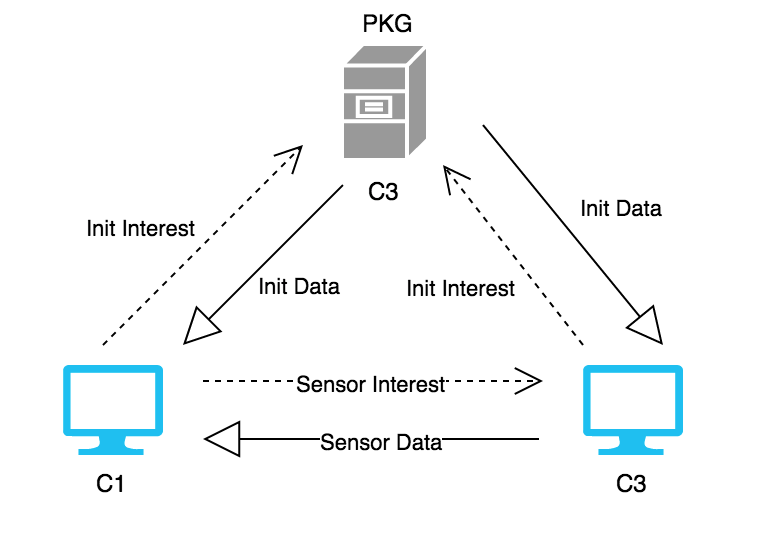
\includegraphics[width=1\textwidth]{hss-testbed.png}
  \caption[HSS testing - computer topology]{Health Sensor System implementation tested over two computer. 
  C3 runs two nodes, i.e. the PKG and one device. 
  C1 runs a second device.}
  \label{fig:hss-testbed}
\end{figure}

\section{NDN Testbed}
The \gls{NDN} testbed is a network of \gls{NDN} nodes created for research purpose. 
\gls{ntnu} joined the testbed contributing with the 24\textsuperscript{th} node in the NDN testbed.
The map of the NDN testbed is shown in~\autoref{fig:ndn-map}.

\begin{figure}[ht]
  \centering
  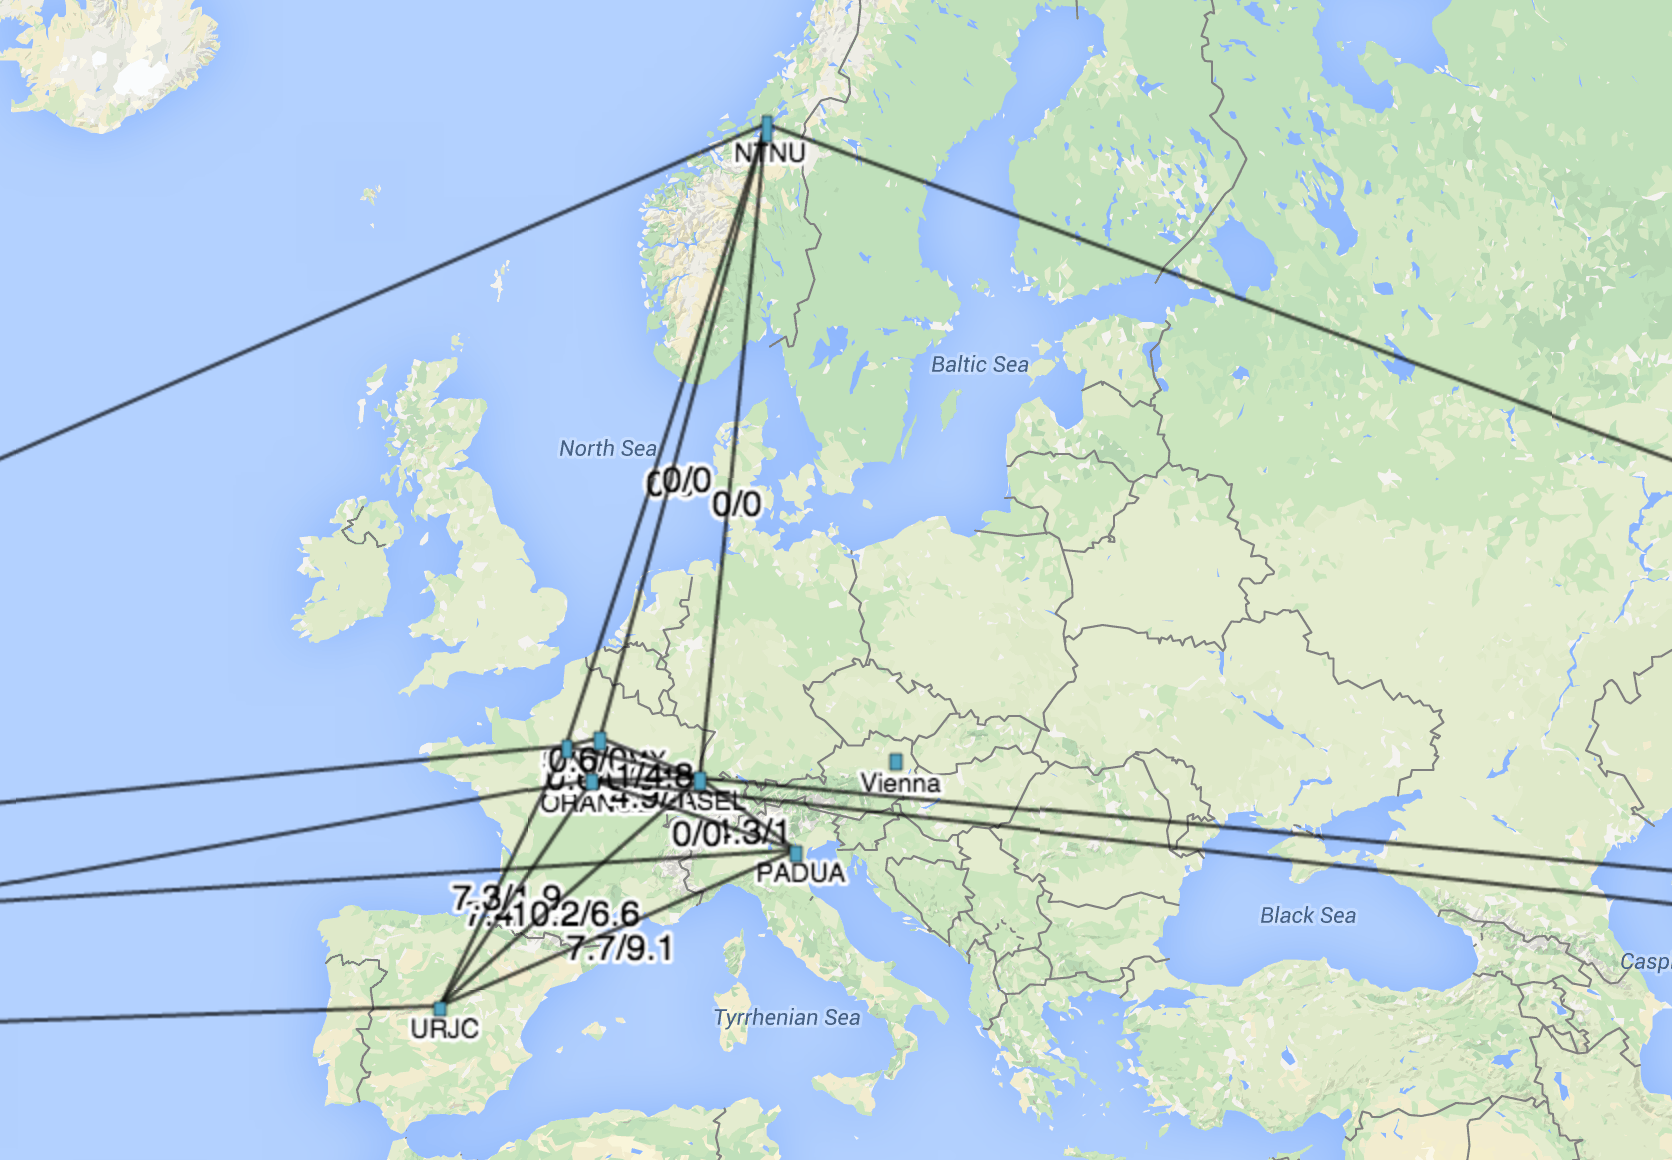
\includegraphics[width=1\textwidth]{ndn-map.png}
  \caption[NDN Testbed map]{NDN Testbed Map}
  \label{fig:ndn-map}
\end{figure}
